

The Acquisition Board's external interface is a bidirectional 8 MHz fiber-optic link over Agilent's 1mm plastic optical fiber. Both the TX and RX streams are encoded using 8b/10b encoding. 

\section{Modes}
The acquisition board has four modes of operation, designed to set the internal state and prevent accidental configuration modification during operation. 

\subsection{Normal acquisition mode}
Mode 0 is the normal acquisition mode; in this mode all 10 channels are sampled at the full normal sampling rate and the data is transmitted over the 8b/10b bus using the standard Encoding Scheme. In this mode, gain and hardware filter settings can be changed, but nothing else. 

\subsection{Offset disable mode}
Offset disable mode disables the internal offset

this is the only mode in which values can be written to the offset locations in the EEPROM



\subsection{input disable mode}
disables input
gain etc have no effect
let you run the samplebuffer


\subsection{raw mode}
just outputs daw data, 192ksps.

\section{Fiber IO}
The Acqboard transmits an 8b/10b-encoded frame of 24 bytes, preceeded by the K28.5 comma character. The nominal frame transmission is as follows:

\begin{figure}[h!]
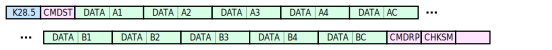
\includegraphics[width=6in]{txpacket.svg}
\end{figure}

CMDST is a 3-bit field; CMDST[1:0] are the mode numbers; CMDST[0] is high \textit{after we have just switched into this mode, while this mode is loading.} Modes load because they need to read data from the EEPROM, etc. 

Every command sent has a 4-bit command id (CMDID); when a command is \textit{done executing} the output command id is changed to reflect this. CMDRP is the command response field; CMDRP[4:1] are the bits of the most-recently executed CMDID; CMDRP[0] tells whether or not this command was successful. 

The data fields are 1.15-bit twos-complement fixed point samples from their corresponding ADCs; they are transmitted MSB first. 

Normally, the acqboard receives a stream of valid 8b/10b encoded zeros; a new command is signalled by the presence of the comma character in the data stream followed by a packet which looks as follows:

\begin{figure}[h!]
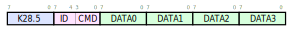
\includegraphics[width=4in]{rxpacket.svg}
\end{figure}

\section{Commands}

The following commands are valid in any mode

\subsection{Universal Commands}

\subsubsection{Switch Mode}
\begin{figure}[h!]
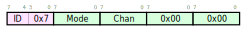
\includegraphics[width=4in]{switchmode.cmd.svg}
\end{figure}

Switch the current acqboard mode to \textsc{mode}. If changing to the RAW mode, the \textsc{chan} field is the 4-bit number of the raw channel you are reading from -- otherwise the field is ignored. 

Note that some mode transitions can take up to 300 ms; during this time the transmitted packet's CMDST will reflect the new mode, but the ``loading'' bit will be set until the mode has been entered. Only once loading is completed will the CMDID be updated. 

\subsubsection{Set Gain}
\begin{figure}[h!]
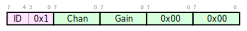
\includegraphics[width=4in]{setgain.cmd.svg}
\end{figure}

Sets the gain of channel \textsc{Chan} to one of the preset gain values \textsc{Gain}. Valid in all modes. 

\subsubsection{Set Input}
\begin{figure}[h!]
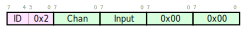
\includegraphics[width=4in]{setinput.cmd.svg}
\end{figure}

Select which of the four channels will be used for tetrode a and B's continuous channel. 

\subsubsection{High Pass Filter Enable}
\begin{figure}[h!]
\includegraphics[width=4in]{setfilter.cmd.svg}
\end{figure}

Enable (\textsc{filter}= 1) or disable (\textsc{filter}=0) the high pass filter on channel \textsc{chan}. 


\subsection{Mode 1 Commands}
\subsubsection{Write offset}
\begin{figure}[h!]
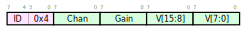
\includegraphics[width=4in]{writeos.cmd.svg}
\end{figure}

This command writes the 16-bit twos-complement value in V as the digital offset for channel \textsc{chan} when the gain on that channel is set to \textsc{gain}. This is only valid in offset-disable mode as to properly measure the zero offsets you'd need to have offsets disabled. 

\subsection{Mode 2 Commands}
\subsubsection{Write filter}
\begin{figure}[h!]
\includegraphics[width=4in]{writefil.cmd.svg}
\end{figure}

This command writes the 22-bit twos-complement value in V as the \textsc{addr}th coeffiient for the low-pass filter. 

\subsubsection{Write Sample Buffer}
\begin{figure}[h!]
\includegraphics[width=4in]{writesamp.cmd.svg}
\end{figure}

This command writes the 16-bit twos-complement value in V as the \textsc{addr}th sample in the no-input sample buffer. 




